\documentclass{article}
\usepackage[utf8]{inputenc}
\usepackage[english]{babel}
\usepackage[font=small,labelfont=bf]{caption}
\usepackage{geometry}
\usepackage{natbib}
\usepackage{pxfonts}
\usepackage{graphicx}
% \usepackage{amsmath}
% \newcommand{\rpm}{\raisebox{.2ex}{$\scriptstyle\pm$}}
% \DeclareMathOperator*{\argmax}{arg\,max}

% \title{Capturing the geometric structure of our experiences and how we remember them}
\title{The fundamental shape of dynamic experiences is preserved in episodic memory}
\author{Andrew C. Heusser \& Jeremy R. Manning}
% \affiliation{Dartmouth College}

\bibliographystyle{apa}

\begin{document}
\maketitle

\section{Abstract}
{
The human memory system is adept at cataloging the rich dynamics of ongoing experience. However, traditional trial-based memory experiments cannot capture these dynamics, and therefore cannot be used to study them.  By constraining participants' experiences in an experiment to occur in temporally discrete trials (and often arranged in a randomized order) the temporal, contextual, and emotional structure of those in-lab experiences necessarily differ from the naturalistic experiences we encounter in everyday life.  Here we investigate how people verbally recall continuous videos by characterizing and relating the thematic dynamics, or ``trajectories,'' of the stimulus and participants' recalls.  Unlike trial-based studies of memory wherein participants attempt to recall the precise stimuli they encounter, naturalistic recall entails capturing the fundamental geometric components of the stimulus topic trajectory.  The precise words participants use to describe the stimulus, and the level of detail and number of distinct events they recall, vary considerably across participants.  Nevertheless, the majority of participants' recall narratives captured the fundamental ``shape'' of the original stimulus.  These findings provide a window into which aspects of naturalistic experiences must be preserved, and which might be more flexible, in considering whether and how those experiences are remembered.

\section{Introduction}

What does it mean to \textit{remember} something? In traditional episodic memory experiments \citep[e.g., list-learning or trial-based experiments;][]{Murd62a, Kaha96}, remembering is often cast as a binary operation: either an item is recalled or it isn't. More nuanced studies might incorporate self-reported confidence measures as a proxy for memory strength, or ask participants to discriminate between ``recollecting'' an experience or a feeling of ``familiarity'' \citep{Yone02}. However, characterizing and evaluating memory in more realistic contexts (e.g., telling a story to a friend about a recent vacation) is much more nuanced. Real-world recall is continuous, rather than binary.  The specific words used to describe an experience have very little bearing on whether the experience is considered to have been ``remembered.''  Further, one might remember the gist of an experience but forget (or neglect to recount) particular details.  Or different people who share an experience might recount the experience with a similar level of detail, but the specific details that were remembered might vary across people.  Which aspects of those recollections should be considered fundamental, and which are extraneous to the main story?

A defining feature of naturalistic experiences is the temporal structure with which they unfold. Our experiences in the real world are typically autocorrelated in space and time on short timescales. In other words, the contents of an experience are often similar from moment to moment and change gradually. For example, many of us spend our mornings/evenings at home and much of our days at work (e.g. an office). While the specific happenings within these contexts differs, they are (usually) highly correlated and predictable over time. Furthermore, our experiences can also be characterized by longer timescale correlations. For example, consider returning to your office after taking a lunch break. The perceptual contexts before and after lunch are highly similar, but separated in time. However, these recurrent and gradually changing temporal dynamics are not typically present in traditional memory studies, but are likely important if we wish to understand how our memory systems remember our everyday experiences.

Despite the continuous and (often) gradually changing nature of naturalistic experiences, prior research suggests that our memories for those same experiences may be more descrete and centered around particular ``events'' \citep{Radv12, RadvZack11, BrunEtal18}. Short timescale autocorrelations in the contents of an experience may cause information to become associatively linked in memory (and thus treated as a single event), while sharp changes (i.e. ``event boundaries'') may segment continuous experiences into events \citep{HeusEtal18, BrunEtal18, Radv12}. There is now compelling evidence that event boundaries can influence memory organization when learning sequences of items \citep{HeusEtal18, DuBrDava13}, during navigation \citep{BrunEtal18}, and narrative comprehension \citep{ZwaaRadv98, EzzyDava11}.  Furthermore, brain activity while viewing naturalistic stimuli displays a block-diagonal structure, and the neurally-derived segments are correlated with judgements of event boundaries \citep{BaldEtal17}.  However, whether people naturally recount their experiences in as events has not been explored.

% We propose that variability in the contents of an experience over time define a ``stimulus-space''. In this space, timepoints where the contents of experience are more similar are represented as points that are closer together. Timepoints with relatively more distinct content are represented further apart. The moment-by-moment flow of content through this space can be represented as a ``stimulus trajectory''.
%
% As a consequence of this structure, we hypothesized that verbally recounted memories for those experiences would mirror this shape.

To study the temporal and semantic aspects of memories for naturalistic experiences, we analyzed an open dataset in which participants view and then verbally recall an episode of the BBC series \textit{Sherlock}  \citep{ChenEtal17}. We Furthermore, we hypothesized that the stimulus To test these hypotheses, we developed a novel computational approach based on topic modeling \citep{BleiEtal03} and hidden Markov models \citep{Rabi89, BaldEtal17} to capture the temporal structure present in naturalistic experiences. We then use this model to characterize the shape of the stimulus as well as verbally recalled memories.

\subsection{Results}

\begin{figure}[t!]
\centering
\includegraphics[width=1\textwidth]{figs/1_analysis_schematic.pdf}
\caption{\small \textbf{Schematic of the analysis approach.} For each scene in the video, text descriptions were generated by hand. Three exemplary time points are displayed here.  Below the video descriptions are text samples from an example participant's verbal recall transcript.  We fit a topic model to the moment-by-moment video text descriptions and transformed participant's verbal recall transcripts using this same model. The bar charts display the resulting topic model weights for the video (in blue) and recall (in orange) for three example topic dimensions.}
\label{fig:schematic}
\end{figure}

\subsubsection{A model to capture the temporal and semantic structure of naturalistic stimuli}
We fit a topic model \citep{BleiEtal03} to (manually annotated) text descriptions of scenes from the video. The text descriptions contained details of the scene such as the characters, location, and a short summary of the scene (see Fig.\ref{fig:schematic} for example text, see \ref{sec:methods} for analysis details). We then transformed the text descriptions using the (same) topic model, resulting in a scenes (1976) by topics (100) matrix, where each row of the matrix represents a probabalistic mixture of topics discovered in that scene (See Fig.\ref{fig:schematic} for example topic vectors). As depicted in Fig.~\ref{fig:model}a, the topic vectors are sparse and change slowly over time. Furthermore, there are clear transitions from one topic `state' to the next, possibly indexing scene transitions in the stimulus. To get a better handle on this temporal structure, we computed a timepoint (1976) by timepoint (1976) correlation matrix of the video model (Fig.~\ref{fig:model}c).  This correlation matrix reveals that the model has a strong, block-diagonal structure. Another noteworthy characteristic is that there is very little correlation between blocks (i.e. the off-diagonal values are small), suggesting the representations of each block are unique and highly descriminable.

\subsubsection{Modeling verbal recall}
After watching the video, participants verbally recalled (in order) as much of the episode as they could.  We used the same topic model (fit with the text descriptions of the video) to transform participants' verbal recall transcripts. The result was a sentences (range: 68 to 294, mean: 131.94) by topics (100) matrix for each participant, where each row represents a probabalistic mixture of topics for a given window of sentences during recall. An example participant's (#13) recall model is plotted in Fig.~\ref{fig:model}c. Like the video model, topic vectors were sparse and changed gradually.  Note that the topics were derived solely from the text descriptions of the video, and so the topic models estimated for recall are dependent on the topics present in the video. This approach effectively projects the participants' verbal recall into the video's `topic space'', allowing us to directly compare them to the video model.

Next, we investigated the temporal structure of the recall matrices. For each participant, we computed a timepoint (68 to 294) by timepoint (68 to 294) correlation matrix from the recall models. An example participant's (\#13) correlation matrix is plotted in Fig.~\ref{fig:model}d). Like the video model, each participant's recall correlation matrix exhibited a strong block-diagonal structure (Supp Fig X). Notably, this suggests that participants recounted the video in discriminable segments, potentially indexing the recall of specific events from the video.

\subsubsection{Segmenting the video and recall models into `events'}
As described above, a striking feature of the video and recall correlation matrices (see Fig.~\ref{fig:model}) is a strong, block structure along the diagonal of the matrices.  We hypothesized that this structure might arise from transient stability in the contents of the video (i.e. ``events''), as well as the subsequent language used to recount each event of the video. If true, we reasoned that it would be possible to identify the specific event a participant is describing by comparing the topic vector for a particular recall ``event'' with the topic vector for each video event. In other words, the video event that is most similar (i.e. correlated) to a particular recall event is the event that the participant is most likely describing.

To test this idea, first we segmented the video and recall models in $k$ events (i.e. states) using a hidden Markov model (~\citep{BaldEtal17}). The algorithm determined 34 events for the video model and a range of values (range: 8-27; mean: 15.41; SD: 5.6) for the recall models (see ~\ref{sec:methods} for details on choosing an optimal $k$ value).  The events discovered for the model and a representative participant (\#13) are highlighted as yellow rectangles outlining blocks along the diagonal of the correlation matrices (Fig.~\ref{fig:model}b,d).

Next, we created a video event model by averaging together neighboring topic vectors that the were classified to be in the same event, resulting in an events (34) by topics (100) matrix (Fig.~\ref{fig:model}e).  We performed the same procedure for the recall matrices (see Fig.~\ref{fig:model}f for example). Then, we computed the correlation between video and recall event models, resulting in a video events (34) by recall events (8-27, depending on the participant) correlation matrix (Fig/~\ref{fig:model}g). These matrices represent the similarity (correlation) between each video event and each recall event (for each participant). To determine which video event a particular recall event was most likely describing, we computed the index of the video event with the highest correlation to the recall event (i.e. the argmax).  This is depicted in Fig.~\ref{fig:model}g as the cells highlighted with a yellow border. Interestingly, our algorithm suggests that the example participant recalled the events largely in order, occasionally skipping a video event.

Then, we computed a group-averaged recall event model and video-recall event correlation matrix. For each participant (and each recall event), we sorted the recall event vectors (across all participants) according to the video event that they were most highly correlated to. We then averaged the recall event vectors within each group. This yielded an average recall event vector for all but one (of 34) video events, since no participant remembered one of the events according to our model. Lastly, we computed an average recall event (34) by video event (34) correlation matrix, and highlighted the cell with the highest correlation value with a yellow border (Fig.~\ref{fig:model}h). Notably, this matrix displayed high correlation values along the diagonal and low correlations in the off-diagonal cells. This suggests that on average, participants were able to recapitulate the events in the episode in a specific, highly descriminable way.
% NOTE: ^ possibly need a null model for the group analysis.  I think it could be to get a result that looks like this even if we scrambled the text. My concern is that I'm grouping the recall events by the video event they were most similar to, and then averaging, which may give rise to a smooth looking plot without any real information there...

\begin{figure}[ht!]
\centering
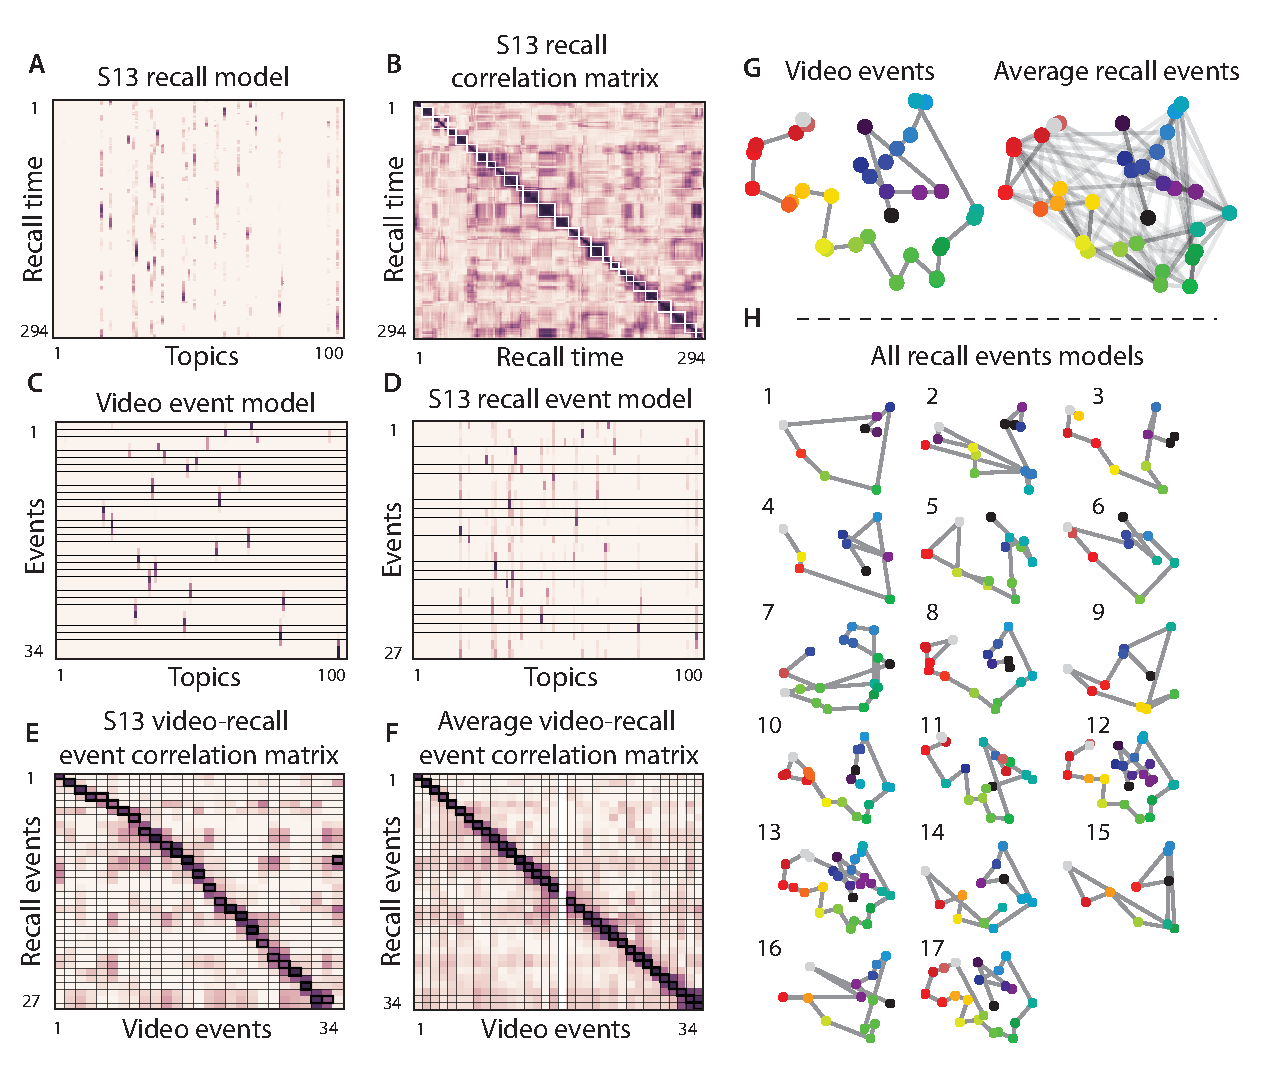
\includegraphics[width=\textwidth]{figs/2_eventseg.pdf}
\caption{\small \textbf{Modelling naturalistic stimuli and recall.} A depiction of our analysis pipeline. For all plots, darker colors indicate greater values and the range of each plot is 0-1.  A). A timepoints (1976) by topics (100) matrix representing the video stimulus.  Each row represents the most likely mixture of topics for a given timepoint (i.e. topic weights). Each column represents a different topic. B). A timepoints (1976) by topics (100) matrix representing participant \#13's recall. C). A viewing-time (1976) by viewing-time (1976) correlation matrix representing the correlation of each moment of the video model with every other moment of the video model. The white boxes represent `events' recovered by a hidden Markov model. D). A recall-time (294 sentences) by recall-time (294) correlation matrix for participant \#13. E). An events (34) by topics (100) matrix where each row represents the average topic vector for each event in the video model.  F). An events (27) by topics (100) matrix where each row represents the average topic vector for each event in participant \#13's recall model. G. A recall events (27) by video events (34) correlation matrix for participant \#13. The cells with a yellow border identify the video event with the highest correlation to a given recall event. F. A group averaged recall events (34) by video events (34) correlation matrix.  The cells with yellow borders are the video event with the highest correlation to a given average recall event.}
\label{fig:model}
\end{figure}


\begin{figure}[t!]
\centering
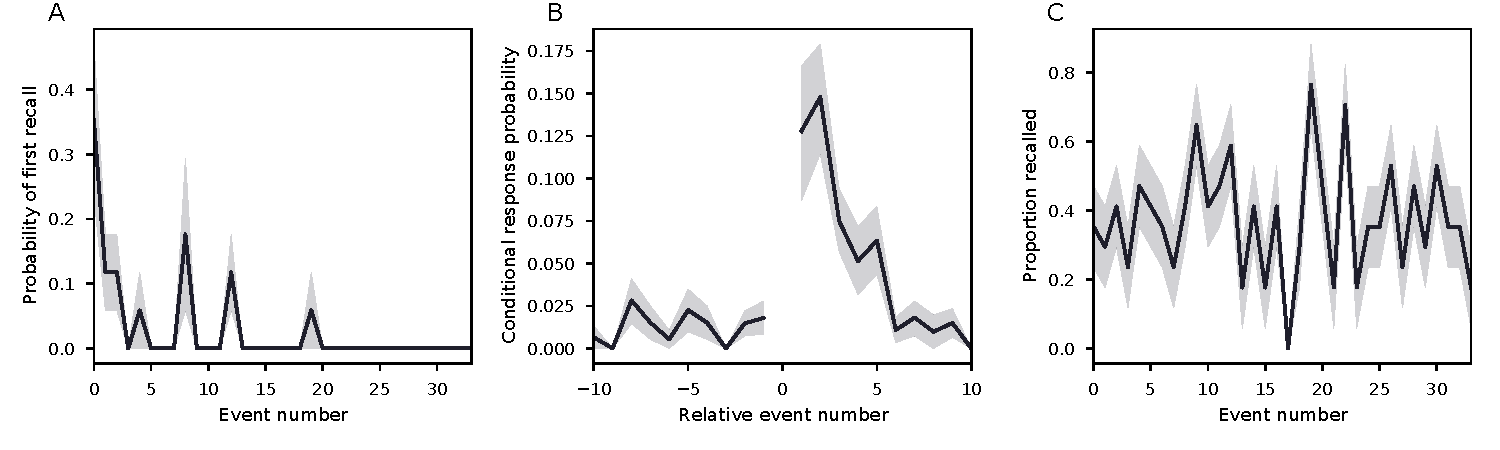
\includegraphics[width=1\textwidth]{figs/3_list_learning.pdf}
\caption{\small \textbf{Naturalistic extensions of classic list-learning memory analyses.} A). The probability of first recall as a function of the serial position of the event during encoding. B). A lag-conditional response probability curve. Given recall of event i, the probability that the next recalled item will be from serial position i +/- lag. C). Proportion of events recalled as a function of serial position. All error bars are the standard error of the mean derived from a bootstrap resampling procedure.}
\label{fig:list-learning}
\end{figure}

\subsubsection{Characterizing naturalistic memory with traditional list-learning analyses}
Just like in a traditional `free-recall' list-learning experiment where participants view a list of words and then verbally recall them, our video-recall matching analysis approach affords us the ability to analyze memory in the same way. The recalled events can be treated as ``items'' analogous to words recalled in a list-learning study. In our first set of analyses, we sought to characterize memory performance/dynamics by extending classic analyses originally designed for list-learning experiments to more naturalistic settings.

First, we asked whether the estimated number of recall events ($k$) by participant was related to hand-annotated accuracy as published in Chen et al. (2017).  We found a strong positive correlation where subjects with a greater number of recall events also had better overall memory performance (Pearson's $r$(16)=.67, $p$=.003). Then, we considered how participants initiated the recall sequence (known in the literature as the `probability of first recall' or `PFR'). This metric quantifies the likelihood of initiating a sequence of recalls based on an item's serial position during encoding. We found that participants tended to initiate their recall sequences with the first few events (Fig.~\ref{fig:list-learning}a), which is qualitatively very similar to previously published list learning experiments (REF). Next, we considered another well-studied memory measure in the list-learning literature, the lag conditional response probability curve (or lag-CRP) ~\citep{Kaha96}. Given the recall of a stimulus in study position $n$, the lag-CRP quantifies the probability that the next item recalled will be of lag $i$. The result suggests a strong bias to transition sequentially events in the forward direction Fig.~\ref{fig:list-learning}b. This can be seen by the high probability values in the lag ~1-5 positions compared to the rest of the transition possibilties. Notably, participants were instructed to recall as much as they could in order, and the shape of this lag-CRP is qualitatively similar to list-learning studies of serial recall (REF), where participants are required to recall lists of words in their serial order. Finally, we assessed memory performance for each event in the video as a function of its serial position during encoding (Fig.~\ref{fig:list-learning}c). We found that there was substantial variability in memory for the different events (STAT?). Furthermore, the shape of the curve is different than what is typically found in list learning experiments (we'll come back to this point in the dicussion).

 We also considered two additional across-participant measures of recall that characterize memory organization: temporal clustering and semantic clustering. Temporal clustering (REF?) measures the extent to which participants tend to cluster recalls of events encoded nearby in time.  For example, if a participant recalled in exact serial order, the score would be 1 whereas if they sequentially recalled randomly positioned items the score would be ~.5.  We found that participants who clustered in time also recalled a greater number of events (Pearson's $r$(16)=.62, $p$=.007). Next, we assessed semantic clustering.  Similar to temporal clustering, semantic clustering measures the extent to which participants cluster their responses by semantic similarity.  We used the topic vector representations of each event as a proxy for semantic information contained in that event.  For each transition, we computed the rank percentile of the of the correlation between the the current event and then next event. For example, if a participant sequentially recalled events where each successive recall was the event that was most semantically similar to the previous, the semantic clustering score would be 1.  If the events were recalled in a random order with respect to semantic information, the clustering score would be ~.5. We found that the semantic clustering score was related to memory performance across participants (Pearson's $r$(16)=.55, $p$=.02).  Thus, participants who organized their recalls with respect to the semantic information contained in the scene had better memory performance.

 \subsubsection{Measuring the quality of naturalistic memories}
 Representing the video and verbal recall as events in `topic space' also affords us the ability to characterize the quality of recall in a more fine-grained and nuanced way than what was previously possible. To quantify the similarity between the video model and individual recall models, we considered a number of novel metrics.  First, we tested whether each participant's recall model matched the movie model in a general sense. To do this, for each participant we filtered the video model to only include the events that the participant remembered. Then, we computed the root mean squared difference (RMSD) between the video model and the recall model. As an example, if the participant remembered all the events in order (with perfect precision), the expected distance value would be 0. However, if they remembered a subset of events, events our of order or with low precision the expected distance would be greater than 0. To assess significance, we performed a permutation test where we circularly shifted the recall model (10000 times) and recomputed the RMSD. The recall model significantly matched the video model for nine of the participants ($p$<.05; participants: 3-4, 8-13, 17 and the p-value for the rest of the participants was less than .25). Furthermore, the RMSD values were significantly correlated to memory performance across participants (Pearson's $r$(16)=-.57, $p$=.016). Thus, a closer match between the video and recall event models was related to better recall performance.

 Next, we tested whether participants who recalled more events were also more precise in their recollections. For each participant, we computed the correlation between each recall event and its matching video event (only for the events which they recalled). This resulted in a single number for each recalled event indexing how similar the recall event was to its matching movie event (i.e the `precision' of the recall). We then averaged the correlations within participant. In line with our prediction, there was a strong correlation between memory performance and precision suggesting that participants who remembered more events also remembered them more veridically (Pearson's $r$(16)=.74, p=.0006). Next, we considered the distinctiveness of each recall event. That is, how uniquely a recall event matched a given video event compared to all other video events. We hypothesized that participants with high memory performance might describe each event in a more distinctive way (relative to those with lower memory performance who might describe events in a more general way). To this end, we computed a `distinctiveness' score for each participant (i.e. 1 - the correlation between a recall event and all non-matching video events).  Then, we averaged this measure over recall events within participant.  We found that participants with higher memory performance also had higher distinctiveness scores (Pearson's $r$(16)=.8, p=.0001).

 Lastly, we tested whether participants with better memory performance were also more likely to remember the events in order.  For each participant, we computed the Spearman rank correlation between the order of events that the participant recalled and the actual order of events (filtering events that were actually recalled).  We found that participants who recalled more events also recalled more of them in order (Pearson's $r$(16)=.5, p=.04). In summary, we found that better memory performance was associated with more precise and distinctive recall.

\subsubsection{The fundamental shape of an experience is preserved in recall}
The analyses described in the previous sections are useful in that they allow us to quantify memory dynamics for naturalistic stimuli in a way that is comparable to a vast literature on trial-based list-learning experiments. However, these methods fail to capture the rich temporal structure present in naturalistic stimuli and associated recall of those experiences. Thus, our next set of analyses test whether the ``shape'' of an experience is preserved in memory. We hypothesized that despite substantial individual variability in the precision and amount of content recalled across by participants, the overall shape of the episode would be recapitulated by the majority of participants.

\begin{figure}[t!]
\centering
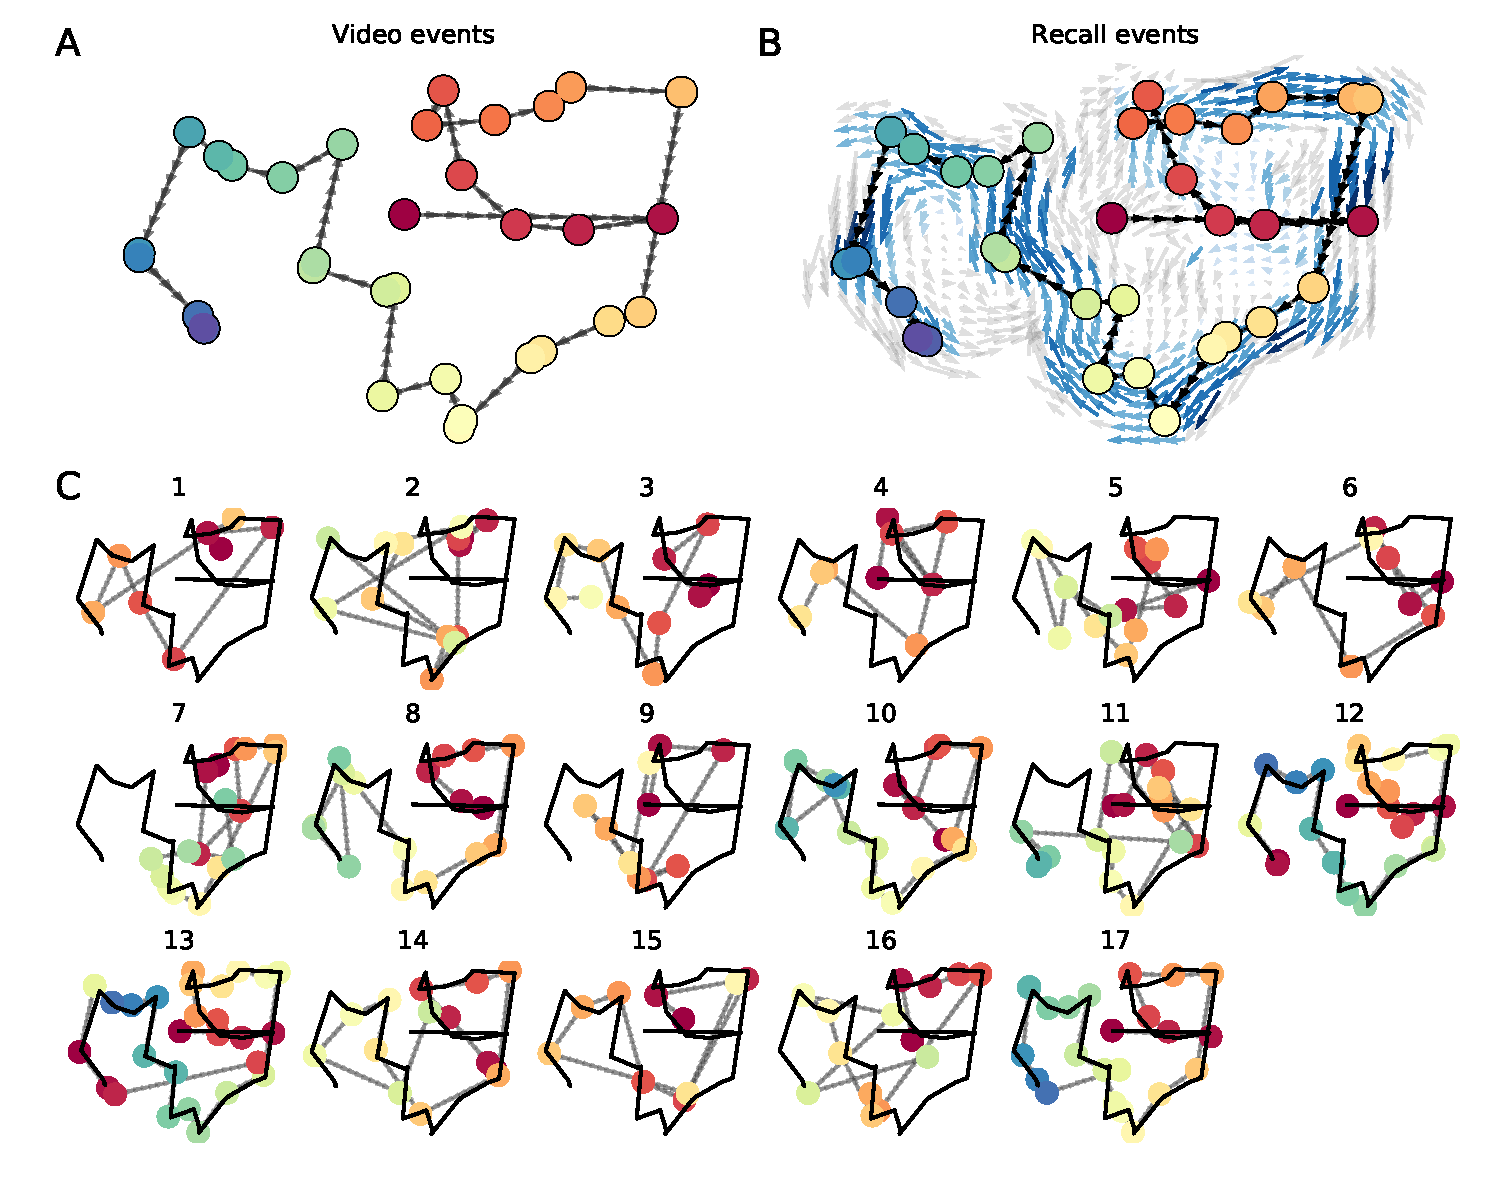
\includegraphics[width=1\textwidth]{figs/4_trajectory.pdf}
\caption{\small \textbf{Video and recall trajectory plots.} A). 2-dimensional embedding of the video events model. The arrows indicate the forward direction of the video events. B). 2-dimensional embedding of the average recall events model.  The colors refer to the most similar video events. The directional lines connecting the points represent the true video event order. The arrows represent the average direction of all recall event transitions (i.e. a line segment connecting two consecutive recall event vectors) that intersected a box (width=.25) centered on the origin of the arrow.
\label{fig:trajectory}
\end{figure}

To visualize the relationship between the video and recall event models, we embedded the video and average recall models into a 2D space (using the UMAP dimensionality reduction algorithm, for details see \ref{sec:methods}) where the points represent video/recall events and the distance between them represents their similarity in ``topic space'' (Fig.~\ref{fig:trajectory}a). (Note that all analyses are performed in the original 100 dimensional space.) We computed the group average transition probabilities from each event to each other event and plotted the values as lines where the tranparency is proportional to the probability of the transition (Fig.~\ref{fig:trajectory}b).  We observed that the two models have a very similar temporal evolution and geometric structure, and the transition probabilities tend to be strongest between events that occured sequentially (or nearby) in time.

\begin{figure}[th!]
\centering
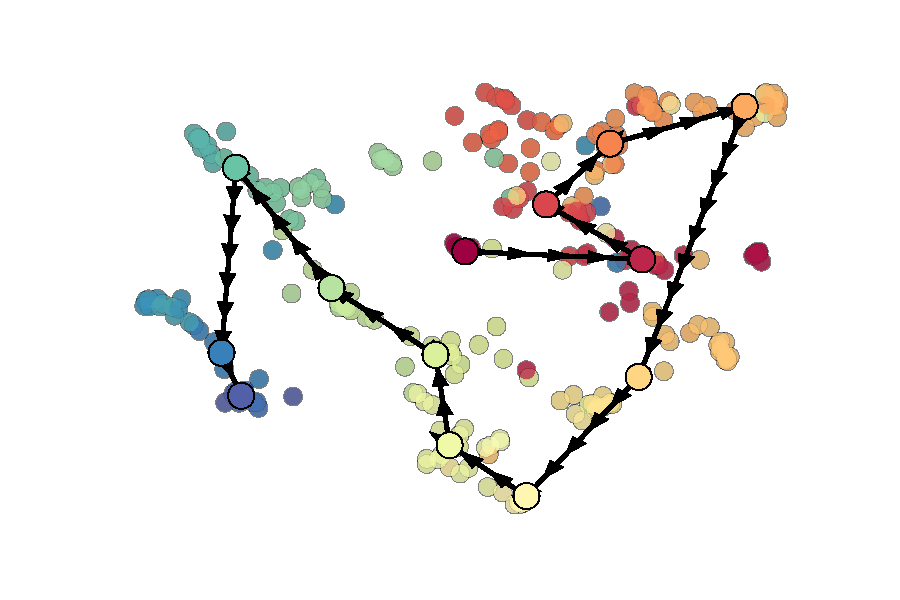
\includegraphics[width=1\textwidth]{figs/5_linesegs.pdf}
\caption{\small \textbf{Recall shape analysis and video/recall content.} A 2-dimensional embedding of the best fitting line segment model.  The points outlined in black represent and connected by black line segments represent the critical recall events (or ``hinge-points'') of the best fitting model colored according to their matching video event.  The points not outlined in black are individual participant recall event topic vectors colored by the most similar video event. The kernel density plot represents the distribution across all points.  The word clouds for hinge-point (left: video; right: recall) were created by plotting the top 100 words from topic model that were ``activated'' during a particular event.}
\label{fig:linesegs}
\end{figure}

To test the observation that participants' recall trajectories generally matched the shape of the video trajectory, we fit participants' recall data to a model comprised of $n$ line segments that were connected by a subset of the average recall event coordinates. We fixed the endpoints of the model at the average first and last recall event, but fit the placement/length of rest of the line segments to the data. Using a cross-validated model fitting procedure (see ~\ref{sec:methods} for details), we searched for the optimal number of line segments. The best fitting model (12 line segments) can be seen in Fig.~\ref{fig:linesegs}. This model represents the set of consecutive line segments that best describe all participants recall event models. Notably, the optimal model comprises a subset of the total recall events (~roughly 1/3). % include a measure of the variance described by the model?

We hypothesized that the points connecting the line segments (referred to as ``hinge-points'') represent critical scenes in the storyline. To visualize the semantic content of each hinge-point, we created wordles from the average topic vectors for each video event (left side), where the size of the word is proportional to its ``activation'' in the video event relative to other video events (Fig.~\ref{fig:linesegs}, see ~\ref{sec:methods} for analysis details). We performed the same analysis for the average recall topic vectors (right side). Notably, the text in the wordles is distinct across the hinge-points, but but similar between video and recall within hinge-point.

\section{Methods}
\label{sec:methods}

\subsection{Participants and Experimental Design}
How much detail here? or just point to janice's paper?

\subsubsection{Fitting the topic model to the video text and recall transcripts}
A topic model was used to estimate the most likely mixture of topics for a given sample of text. First, the video was manually segmented into 1000 scenes, and a collection of descriptive features was manually transcribed. For each scene, we considered the following features: scene details (i.e. a sentence or two describing what happened in that scene, space (indoor or outdoor), name of all the characters in the scene, name of the character in focus, name of the character speaking, location, camera angle, music presence, and words on the screen. We concatenated the text for all of these features within each segment, creating a 'bag of words' describing each scene. We then transformed the text descriptions into overlapping windows of 50 scene segments. For example, the first text sample comprised the text from the first 50 segments, the second comprised the text from n+1:n+51, and so on. We trained our model using these overlapping text samples using scikit-learn's (version 0.19.1) `CountVectorizer' and `LatentDirichletAllocation' classes.  First, the text was transformed into a vector of word counts (default parameters). This gave a word count vector for each scene in the video.  Then, the word count vectors were used to fit a topic model (\# of topics=100, method=batch). We transformed the text descriptions using the model resulting in a scenes (1000) by topics (100) matrix. The scene descriptions often spanned multiple timepoints (i.e. TRs). To account for this, we expanded the video model by copying the rows of the model for as many timepoints that the scene description spanned. After this expansion, the shape of the model was the length of the duration of the video (1976 TRs).

To create the recall models, for each participant we tokenized the recall transcript into a list of sentences and then mapped the list to overlapping windows of 10 sentences.  We transformed the list of overlapping recall sentences using the model that was trained on the video text (as described in the paragraph above). The result of this was a sentences (range: 68-294) by topics (100) matrix for each participant that represented the most likely mixture of topics for a given chunk of sentences.

\subsubsection{Extracting events using a hidden Markov model}
The topic model timepoint-by-timepoint correlation matrices all exhibited a block-diagonal structure (with small off-diagonal values), suggesting that the models were comprised of a number of sequential `states' (or events). To capture this structure, we fit the video and each recall model using a hidden Markov model (HMM). Given a number of states or events ($k$), the HMM recovers a set of labels that segments consecutive timepoints into $k$ events (REF markov paper). To implement this analysis, we used the Brainiak toolbox \citep{BaldEtal17}.

Our metric for choosing the `best fitting' HMM was to choose the model with the $k$ value that maximized the ratio of the average `within-event' correlation values (i.e. the correlation values for blocks of consecutive timepoints the model identified as one event) and the average `across-event' correlation (i.e. the rest of the correlation values). Additionally, we included a penalty parameter that was proportional to the smoothing of the model that preferred models with smaller $k$ values. We chose $k$ values separately for the video model and for each recall model.  Then, using the best $k$ values, We fit a separate HMM for each topic model. Finally, we averaged over timepoints identified to be in the same event resulting in a $k$ events by 100 topics matrix for the video model and each of the recall models.
%
\subsubsection{Matching recall events to video events}
To figure out which video event each recall event referred to, we correlated the video events model and each recall events model. This resulted in a video events (34) by recall events (8-27) correlation matrix (for each participant) which contains the similarity between each video event and each recall event.  To find the most likely video event that a given recall event referred to, we computed the argmax over the columns of this matrix.  The result was a list of video event indices for each participant. These indices are analogous to the values found in a ``recall matrix'' from a free recall list learning experiment, but represent the recall of particular events (instead of words, for example).
%
\subsubsection{Characterizing memory performance using traditional approaches.}

\textbf{Overall Accuracy.}  To get an overall measure of the quantity of information recalled, we computed the proportion of sucessfully recalled events by counting the number of unique recall events identified by the HMM model and dividing by the total number of video events.  We performed this analysis for each participant separately.

\textbf{Probability of first recall (PFR).}  The (PFR) analysis represents the probability that an item will be recalled first as a function of its serial position during encoding. We initialized a \# of participants (17) by \# of video events (34) matrix. Then for each participant, we found the index of the video event that was recalled first and filled in that index in the matrix with a 1.  Finally, we averaged over the rows of the matrix, resulting in a 1 by 34 array representing the proportion of subject that recalled an event as a function of serial position during encoding.

\textbf{Lag conditional probability curve (lag-CRP).} The lag-CRP represents the probability that the next item recalled will be of lag $i$ from the just recalled item. For each recall transition, we computed the lag between the current recall event and the next recall event, normalizing by the total number of possible transitions.  This resulted in a \# of participants (17) by lags (-33:+33) matrix. We averaged over the rows of this matrix to get a group-averaged lag-CRP.

\textbf{Serial position curve (SPC).} The SPC represents the proportion of participants that remember an item as a function of its serial position during encoding. We initialized a \# of participants (17) by \# of video events (34) matrix. Then, for each recall event (and each participant), we found the index of the video event that was recalled and filled it in with a 1. This resulted in a matrix where 1s indicate the successful recall of an event in serial position $n$ and zeros indicate the lack of recall for that event.  Lastly, we averaged over the rows of the matrix to get a 1 by 34 array representing the proportion of subjects that recalled an event as a function of its serial position.

\textbf{Temporal clustering.} Temporal clustering measures the extent to which participants group their recall responses according to encoding position. For instance, if the participant recalled each item in the presentation order, this would result in a score of 1. If the participant recalled randomly with respect to presentation order, this would result in a score of ~.5.  For each event transition (and separately for each participant), we computed the rank similarity (euclidean distance) between the presentation position  of the current and next recall events. The scores were then averaged within participant to get a single number representing the extent of temporal clustering exhibited by a given participant.

\textbf{Semantic clustering.} Similar to temporal clustering, semantic clustering measures the extent to which participants group their recall responses according to semantic similarity. Here, we are using the topic vectors for each event as a proxy for its semantic content. Thus, similarity between the semantic content for two events can be computed by correlating their respective topic vectors.  For instance, if each consecutive recall was the next most similar event (in terms of its s), this would result in a score of ~1. If the participant recalled randomly with respect to semantic similarity, this would result in a score of ~.5.  For each event transition (and separately for each participant), we computed the rank similarity (correlation distance) between the current recall event and the next recall event. The scores were then averaged within participant to get a single number representing the extent of semantic clustering exhibited by a given participant.

\subsubsection{Visualizing the video and recall event models.}

To better understand the temporal structure of the video event model (34 events by 100 topics) and the recall event models (8-27 events by 100 topics), we used a technique called UMAP to reduce the ``topic-space'' from 100 dimensions down to 2 dimensions (REF). UMAP is a nonlinear dimensionality reduction technique which models the manifold of the data with a fuzzy topological structure, and then searches for a (2D) projection of the data that has the closest equivalent fuzzy topological structure. We concatenated (vertically stacked) all event models (video, average recall, and individual recall), and then fit and transformed all of the models at once. This assured that the models were projected into the same space.

\subsubsection{Vector field analysis.}
To quantify (and visualize) the flow of recall from event to event, we performed a vector field analysis.  We tiled the 2D topic space (x, y: -6 to 6 by .25) with an evenly spaced grid. For each grid point, we drew a square around the point (height/width=.5).  Then, we tested whether any line segments (formed by event recall transitions) passed through this area of the topic space.  For example, say that a participant transitioned from recalling event 2 to event 3. These 2 recall events correspond to 2 points in topic space, and connecting them forms a line segment. We collected all line segments that passed through a given section of topic space (collapsing across participants). To plot the average direction of the line segments (i.e. the arrows for each grid point in ~\ref{fig:trajectory}b), we converted each of them to unit vectors and then averaged. For grid points where the direction was consistent (across all participants contributing to that point), the length of the arrow approaches 1, whereas if the direction was random the length of the arrow approaches 0. Lastly, we converted each unit vector to an angle (in radians) by taking the inverse tangent of the x, y components of the vector. To test whether the distribution of angles was significantly non-uniform (i.e. displayed a preferred direction across participants), we performed a Rayleigh test on the angles (REF). Arrows where the Rayleigh test was significant are displayed in color while non-significant tests are displayed in gray with lower opacity.



% We used a few different metrics to assess memory that were all designed to capture the relationship between the video and recall models.  First, to get a general sense for the match between the video and recall matrices, we vectorized the the matrices and correlated them.  This resulted in a single number representing how well a given participant recalled the video. To get a temporally dynamic measure of memory, for each participant we computed the pairwise correlation between matching video/recall timepoints.  This allowed us to assess memory for individual moments of the video. Finally to get a more nuanced representation of memory for the video, we computed a video/recall model correlation matrix for each participant. These timepoint (1976) by timepoint (1976) matrices represent the correlation between every moment of the video model and every moment of the recall model. To provide some intuition, if a participant recalled every scene at the same rate and in exactly the same order as the video, we would expect high correlation values along the diagonal of this matrix. However, if a participant recalls the scenes out of order, or at different rates for different scenes, this will result in high values off the diagonal.
%
% The only additional constraint we imposed was that there was at least 2 points between each line segment.
% We searched for the optimal number of line segments by iteratively splitting the participants into two groups, fitting the model to the first half and testing the model on the remaining subjects. To compute fit to the model, for each recall event (a 1 by 100 topics vector) we computed the nearest line segment and then calculated the mean squared distance averaging over all events and all participants (in the sample). We repeated this 20 times using 1-10
%
% \subsubsection{Bridging between the stimulus and recall}
% The participants in this study were instructed to recall as much of the episode as they could in the order it happened.  Thus, we hypothesized that the recall models should resemble the video model to the extent that participants followed these instructions and had reasonably good memory accuracy. To test whether this was true, we correlated each moment of the video model with each moment of each participants' resampled recall model. We then averaged these matrices together to get a single group averaged matrix.  The result was a viewing time (1976) by recall time (1976) correlation matrix representing the average relationship between every moment of the movie and recall models (Fig.~\ref{fig:model}e). Notably, we observe significant correlation values (p<.05, permutation test described in \ref{sec:methods}) primarily along the diagonal, suggesting that our model captures the fact that participants recalled the episode in order. We also visualized this effect by projecting the matrices into a 3D space (reduced using Spectral Embedding [cite]) where the proximity of the trajectories at every timepoint represents how similar the topic vectors were. Visualizing the data in this way makes it clear that the overall shape and correlational structure of the video and average recall matrices is quite similar.

\bibliography{memlab}
\end{document}
